\documentclass[border=10pt]{standalone}
\usepackage{tikz}
\usetikzlibrary{arrows.meta}

\begin{document}
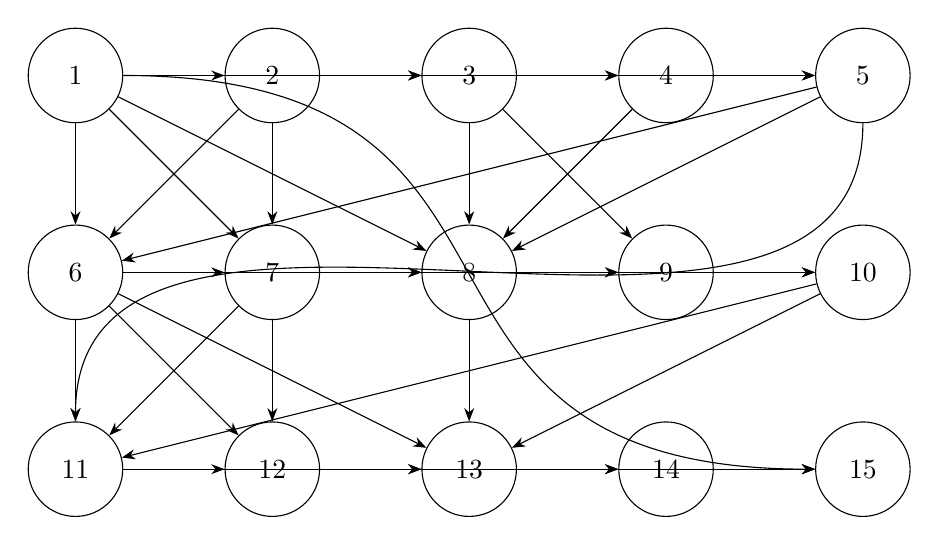
\begin{tikzpicture}[->, >=Stealth,
    every node/.style={circle, draw, minimum size=1.2cm, font=\normalsize}]

  % 15 nodes in 5x3 grid layout
  \foreach \row in {0,1,2} {
    \foreach \col in {0,1,2,3,4} {
      \pgfmathtruncatemacro{\n}{\row*5 + \col + 1}
      \node (\n) at (\col*2.5, -\row*2.5) {\n};
    }
  }

  % Adjacent edges (straight)
  \draw (1) -> (2);
  \draw (2) -> (3);
  \draw (3) -> (4);
  \draw (4) -> (5);
  \draw (5) -> (6);
  \draw (6) -> (7);
  \draw (7) -> (8);
  \draw (8) -> (9);
  \draw (9) -> (10);
  \draw (10) -> (11);
  \draw (11) -> (12);
  \draw (12) -> (13);
  \draw (13) -> (14);
  \draw (14) -> (15);

  % Vertical edges (straight)
  \draw (1) -> (6);
  \draw (2) -> (7);
  \draw (3) -> (8);
  \draw (6) -> (11);
  \draw (7) -> (12);
  \draw (8) -> (13);

  % Skip-one edges (bend to avoid middle node)
  \draw[bend left=30] (1) -> (3);
  \draw[bend left=30] (2) -> (4);
  \draw[bend left=30] (3) -> (5);
  \draw[bend right=30] (6) -> (8);
  \draw[bend right=30] (7) -> (9);
  \draw[bend right=30] (8) -> (10);
  \draw[bend left=30] (11) -> (13);
  \draw[bend left=30] (12) -> (14);
  \draw[bend left=30] (13) -> (15);

  % Diagonal edges (slight bend)
  \draw[bend left=15] (1) -> (7);
  \draw[bend right=15] (2) -> (6);
  \draw[bend left=15] (3) -> (9);
  \draw[bend right=15] (4) -> (8);
  \draw[bend left=15] (6) -> (12);
  \draw[bend right=15] (7) -> (11);

  % Long diagonal (larger bend)
  \draw[bend left=40] (1) -> (8);
  \draw[bend right=40] (5) -> (8);
  \draw[bend left=40] (6) -> (13);
  \draw[bend right=40] (10) -> (13);

  % Cross edges with in/out angles
  \draw[out=0, in=180, looseness=1.5] (1) to (15);
  \draw[out=-90, in=90] (5) to (11);

\end{tikzpicture}
\end{document}
